%set ukuran paper jadi a4 sama 12 pixel font
\documentclass[a4paper,12pt, left=3cm,right=2cm,bottom=2cm, bahasa]{article}
\usepackage{graphicx} % Required for inserting images
\usepackage[utf8]{inputenc}
\usepackage{times}
\usepackage{float}

\usepackage[autostyle]{csquotes}

%hyprlink desuwa
\usepackage{hyperref}
\hypersetup{
    colorlinks,
    citecolor=black,
    filecolor=black,
    linkcolor=black,
    urlcolor=black
}
%ganti jadi roman
\usepackage{times}

%set margin
 \usepackage{geometry}
 \geometry{margin=2cm}

%set bahasa indonesia
%\captionsbahasa
% \usepackage[american]{babel}


%biber dsw
% \usepackage[backend=biber,style=apa, sorting=none]{biblatex}
% \addbibresource{./ref.bib}


%set spacing 1.5
 \usepackage{setspace}
 \onehalfspacing{}
\usepackage{tocloft}

%bikin tabel berwarna
\usepackage[table,xcdraw]{xcolor}
\renewcommand{\cftpartleader}{\cftdotfill{\cftdotsep}}

%daftar pustaka
\renewcommand{\refname}{Daftar Pustaka}

%bikin judul utama centering
\usepackage{titlesec}
\titleformat{\section}[hang]{\normalfont\Large\bfseries}{\thesection}{1em}{\centering}
%idk harus pake date biar gak nongol di title
\date{}

%judul dokumen
\title{Laporan Kunjungan Wawancara\\ Praktikum Pendidikan kewarganegaraan}

\begin{document}

%bikin judul jalan
\maketitle
%bikin page ini ga pake nomor
\thispagestyle{empty}
% logo
\begin{figure}[H]
    \centering
    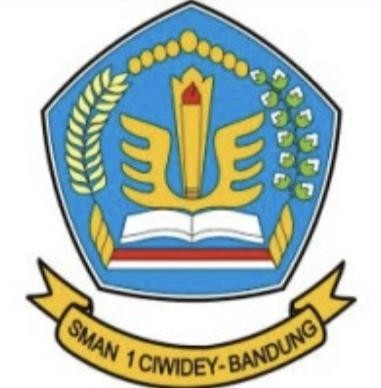
\includegraphics[width=0.3\linewidth]{images/sman1.png}
\end{figure}
%vertical space 2 cm

%nama penulis
\begin{center}
    Kelompok 2 : \\
    \begin{tabular}{ll}
         1.& Hasby Nauril Atoriq  \\
         2.& Rezza Rahmadani \\
         3.& Riana Nur Rahmadina \\
         4.& Hanesty Almaida \\
         5.& Karmila Gunawan \\
         6.& Naysila Zahrotulsita \\
         7.& Novi Aulia Ginarti \\
         8.& Putri Oktaviani \\

    \end{tabular}\\
    \vspace{0.5cm}
    Kelas X-1\\
    \vspace{1cm}
    \textbf{PEMERINTAH DAERAH PROVINSI JAWA BARAT}\\
    \textbf{DINAS PENDIDIKAN}\\
    \textbf{SMA NEGERI 1}
    \textbf{CIWIDEY}\\
    \textbf{2025}
\end{center}
\onehalfspacing{}
%ganti nomor jadi romaj
\pagenumbering{Roman}
\setcounter{section}{1}
\pagebreak

    \section*{DAFTAR ISI}
    \addcontentsline{toc}{section}{\protect\numberline{}DAFTAR ISI}
% \end{center}
\renewcommand{\cftdot}{.}
\renewcommand{\contentsname}{}
\tableofcontents



%\vspace{3cm}
%\section*{DAFTAR PUSTAKA}
%\addcontentsline{toc}{section}{\protect\numberline{}DAFTAR PUSTAKA}
%\medskip
%\printbibliography

\pagebreak
\pagenumbering{arabic}
\setcounter{page}{1}
\setcounter{section}{1}


\section*{BAB I \\PENDAHULUAN}
\addcontentsline{toc}{section}{\protect\numberline{}BAB I PENDAHULUAN}
\subsection{Waktu dan Tempat Kegiatan}
Hari/Tanggal: Selasa, 18 Februari 2025 \\
Waktu: Pukul 13.00–16.00 WIB \\
Lokasi: Balai Desa Ciwidey, Kabupaten Bandung, Jawa Barat \\

%bab 2
\setcounter{subsection}{0}
\setcounter{section}{2}
\section*{BAB II \\ Uraian Hasil Observasi}
\addcontentsline{toc}{section}{\protect\numberline{}BAB II Uraian Hasil Observasi}
\subsection{Demografis Ciwidey}
Ciwidey sebagai wilayah agraris di Kabupaten Bandung memiliki komposisi penduduk yang didominasi oleh Suku Sunda (76,53\%) sebagai kelompok mayoritas, dengan minoritas terbesar berupa Suku Jawa (12,68\%) dan kelompok etnis lain seperti Tionghoa (3,31\%) serta Batak (1,76\%)3. Data keagamaan menunjukkan 92,17\% penduduk beragama Islam, diikuti minoritas Kristen Protestan (5,17\%), Katolik (2,14\%), Buddha (0,44\%), dan Hindu (0,06\%)3. Pola ini merefleksikan dinamika sosial di Jawa Barat secara umum, di mana interaksi antar kelompok dipengaruhi oleh struktur demografis yang hierarkis.
% cite this shit https://p2k.stekom.ac.id/ensiklopedia/Kota_Bandung

\subsection{Adaptasi Kelompok Minoritas}
Kelompok minoritas agama dan etnis di Ciwidey mengembangkan strategi adaptasi melalui integrasi terbatas. Komunitas Tionghoa, misalnya, mempertahankan tradisi budaya seperti perayaan Imlek di ruang privat sambil berpartisipasi dalam kegiatan sosial desa2. Hal ini sejalan dengan penelitian di Jayapura yang menunjukkan bagaimana minoritas membangun identitas ganda: mematuhi norma mayoritas sekaligus memelihara kekhasan kelompok2. Pada komunitas Kristen, pembangunan gereja seringkali terkendala persyaratan administratif, sehingga mereka memanfaatkan rumah warga sebagai tempat ibadah sementara2 \cite{Admin:2005}
% cite this shit https://balitbangdiklat.kemenag.go.id/berita/problem-mayoritas-dan-minoritas-dalam-interaksi-sosial

\subsection{Faktor Penghambat Integrasi}
Observasi Mengungkap tiga tantangan utama:
\begin{enumerate}
  \item Ketimpangan ekonomi: kelompok pendatang seperti etnis Tionghoa mendominasi sektor perdangan, menimbulkan persepsi ketidakadilan di kalangan masyarakat lokal 
  \item Privasi Terbatas: Hunian sementara bagi korban bencana alam (seperti erupsi Gunung Patuha) seringkali tidak memenuhi standar kesehatan dan privasi, mirip dengan kondisi huntara pasca-erupsi Merapi1. Hal ini berpotensi memperparah ketegangan sosial.
  \item Sentimen Lokalisme: Kebijakan otonomi daerah memicu penguatan identitas kesundaan, yang terkadang bertabrakan dengan kepentingan kelompok pendatang
\end{enumerate}

\subsection{Peran faktor sosial}
Tokoh agama dan adat berperan sebagai mediator konflik. Forum Silaturahmi Lintas Iman (FSLI) Ciwidey telah menjadi wadah dialog untuk menyelesaikan sengketa lahan makam antarumat beragama. Mekanisme ini mirip dengan pola kerukunan di Kupang yang mengandalkan kearifan lokal dan figur tokoh2. Namun, efektivitasnya masih terhambat oleh rendahnya partisipasi pemuda dalam kegiatan lintas budaya.
%bab 3
% weird shit, harus pake 0
\setcounter{subsection}{0}
\setcounter{section}{3}
\section*{BAB III \\  Dokumentasi}
\addcontentsline{toc}{section}{\protect\numberline{}BAB III Dokumentasi}
\begin{figure}[H]
  \begin{center}
    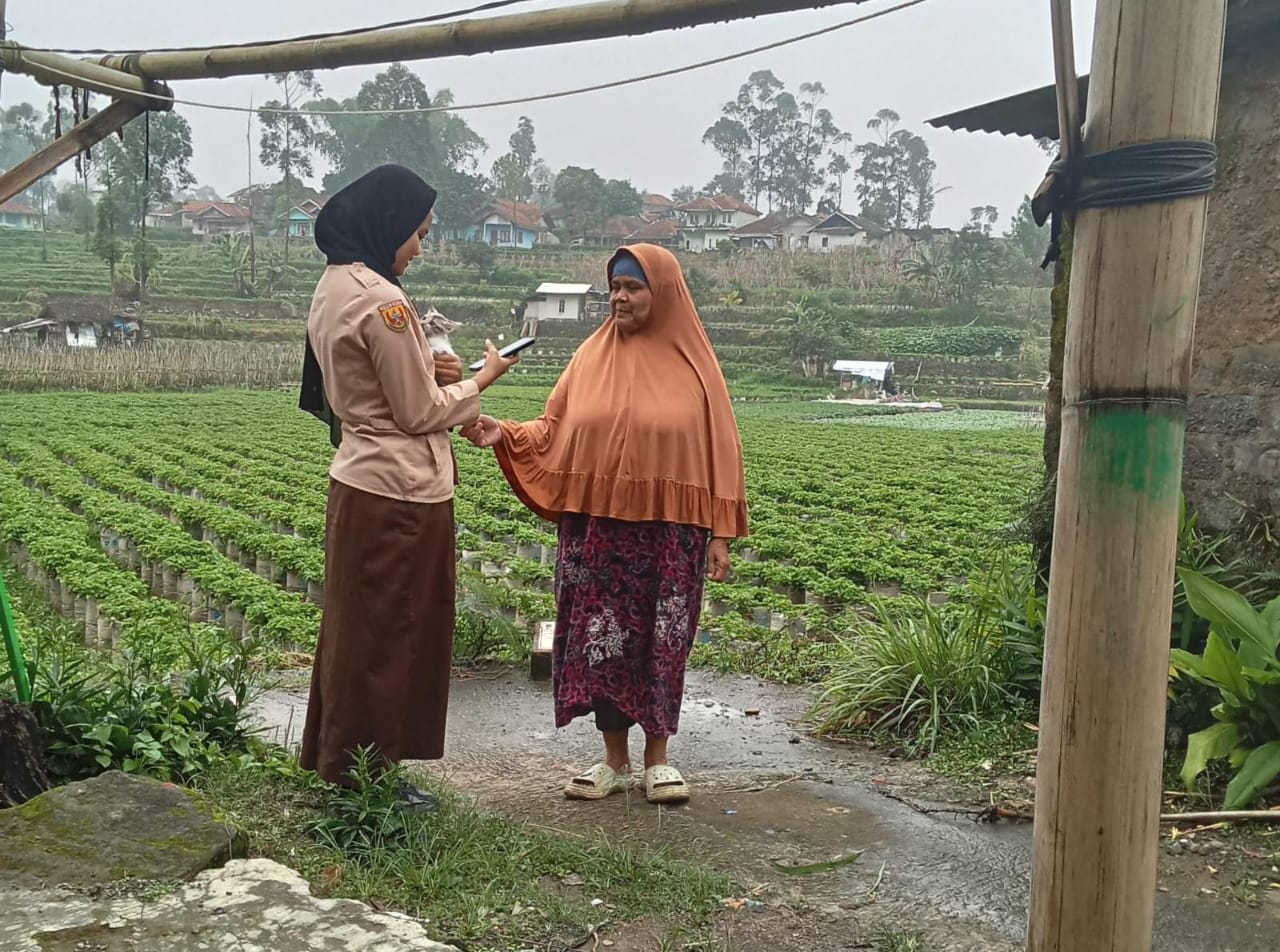
\includegraphics[width=0.4\textwidth]{images/gambar1.jpeg}
  \end{center}
\end{figure}
\begin{figure}[H]

  \begin{center}
    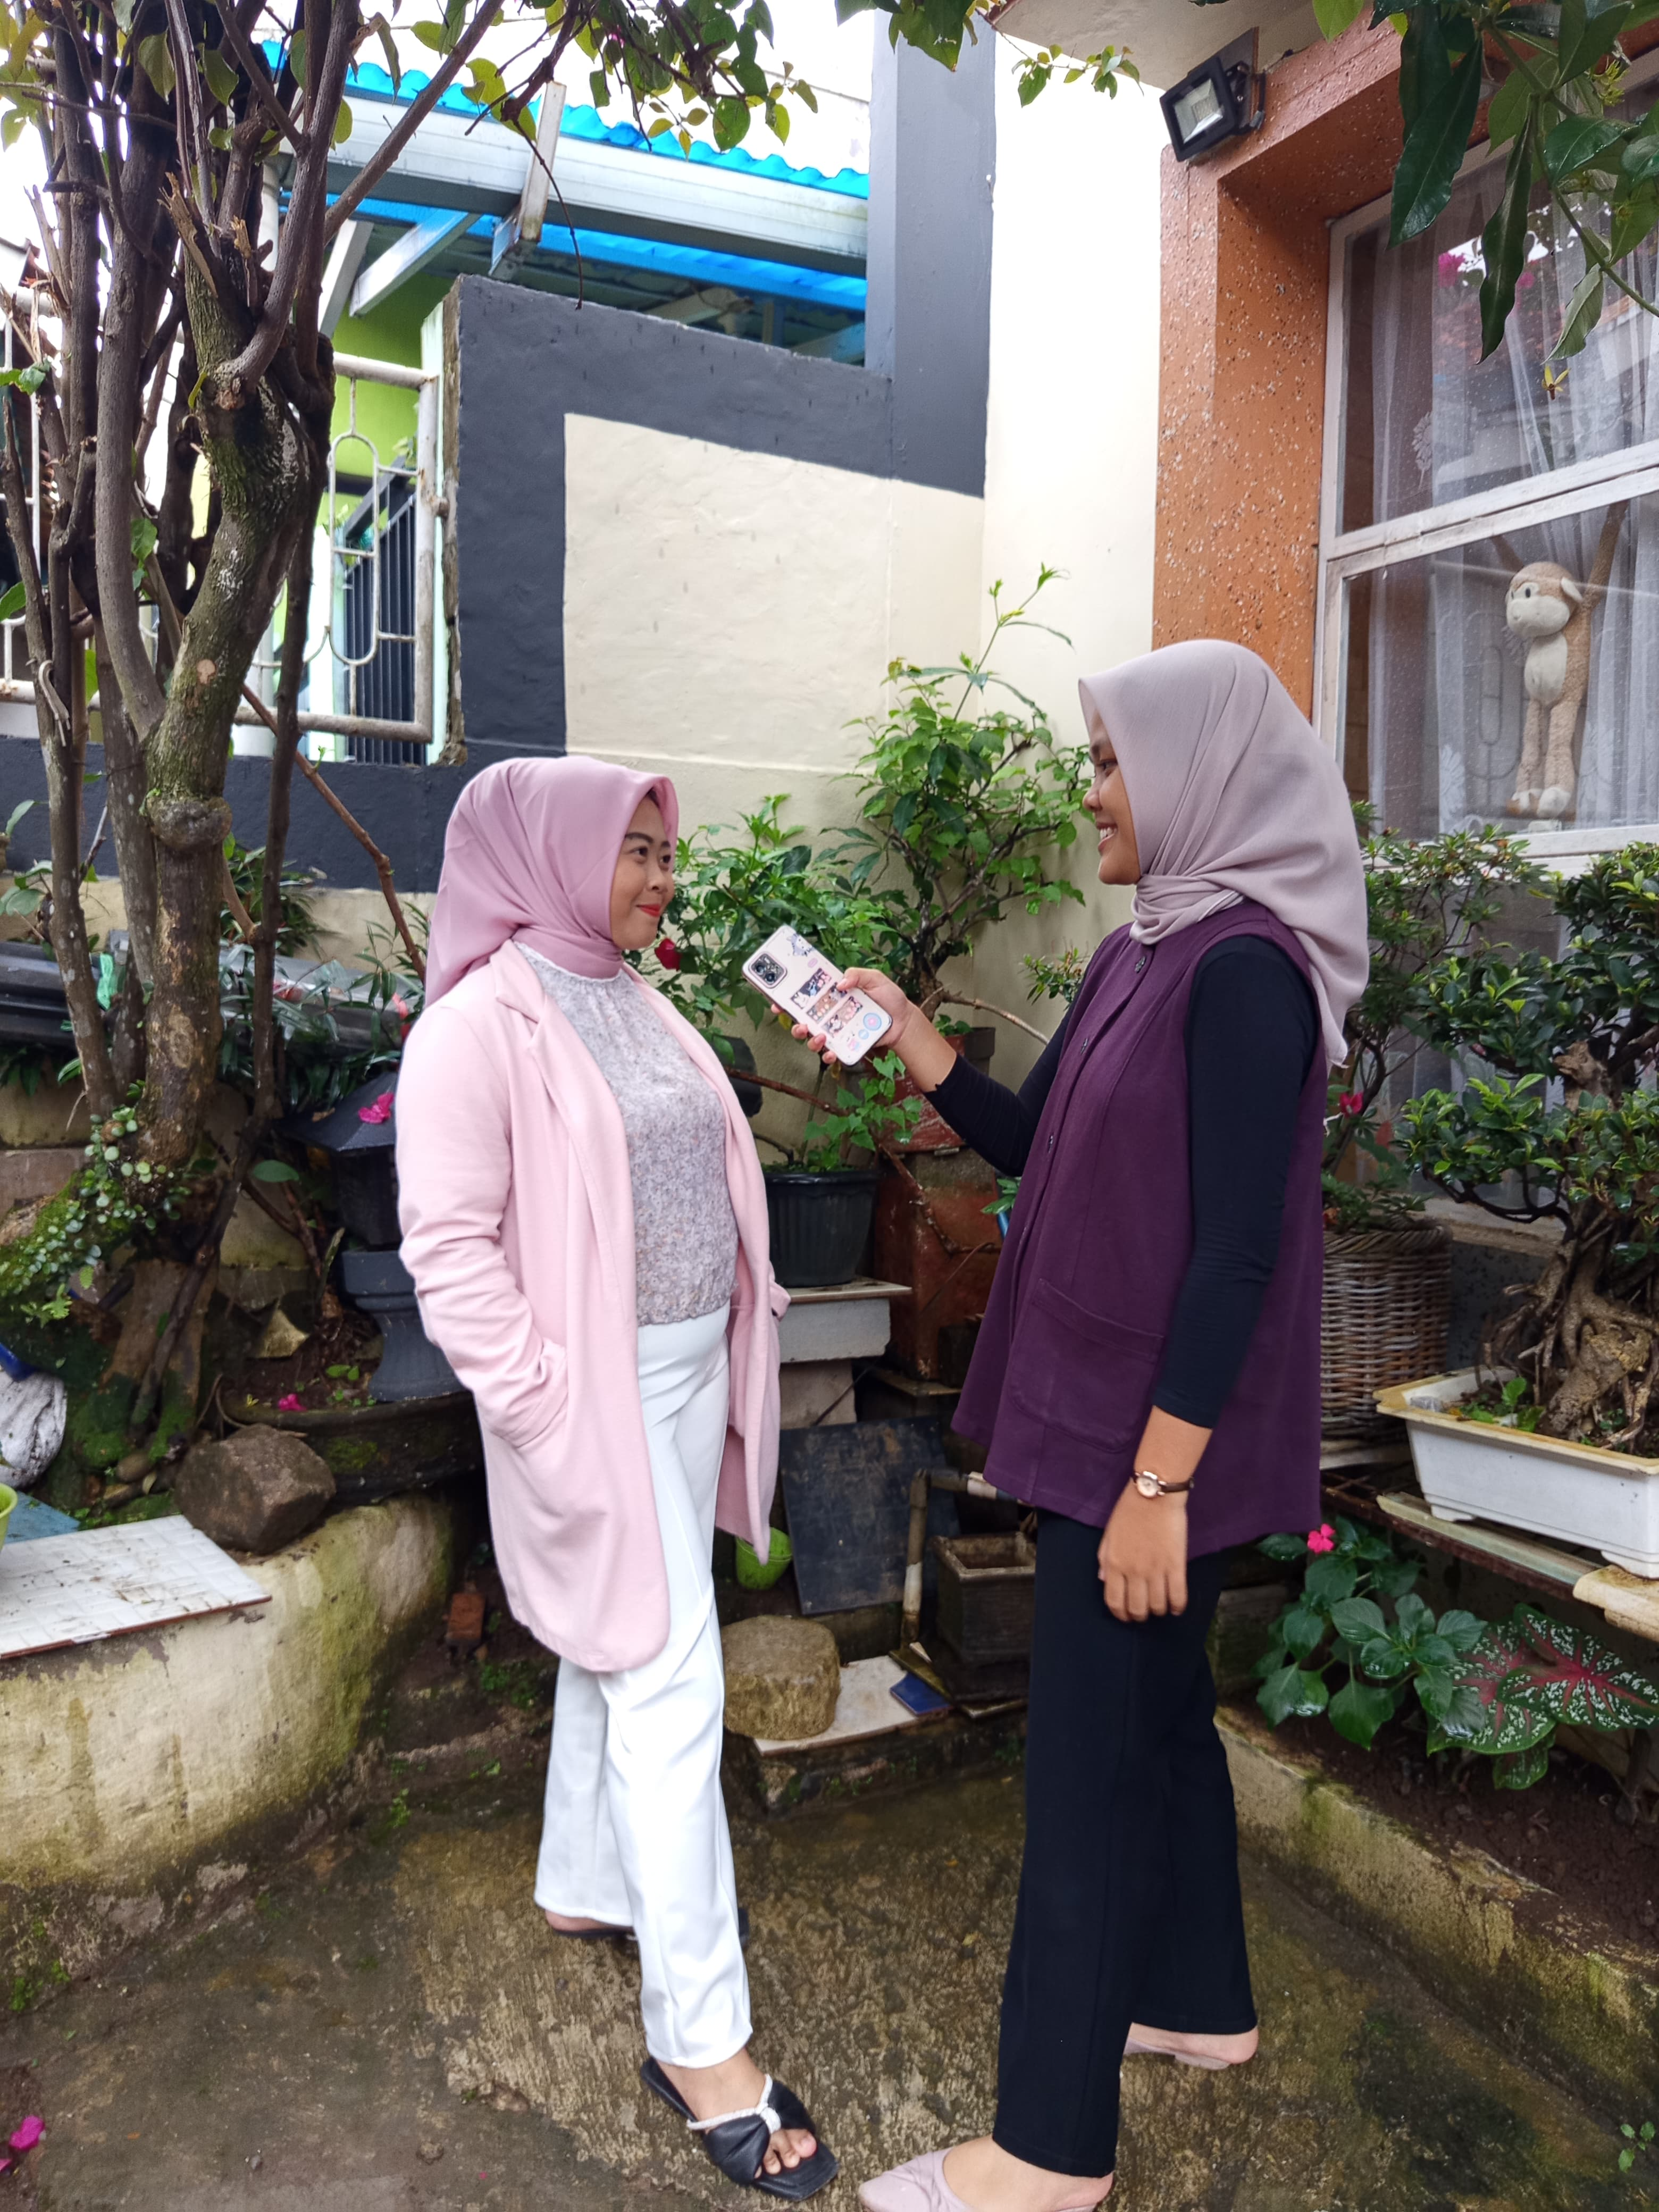
\includegraphics[width=0.4\textwidth]{images/gambar2.jpeg}
  \end{center}
\end{figure}
\begin{figure}[H]

  \begin{center}
    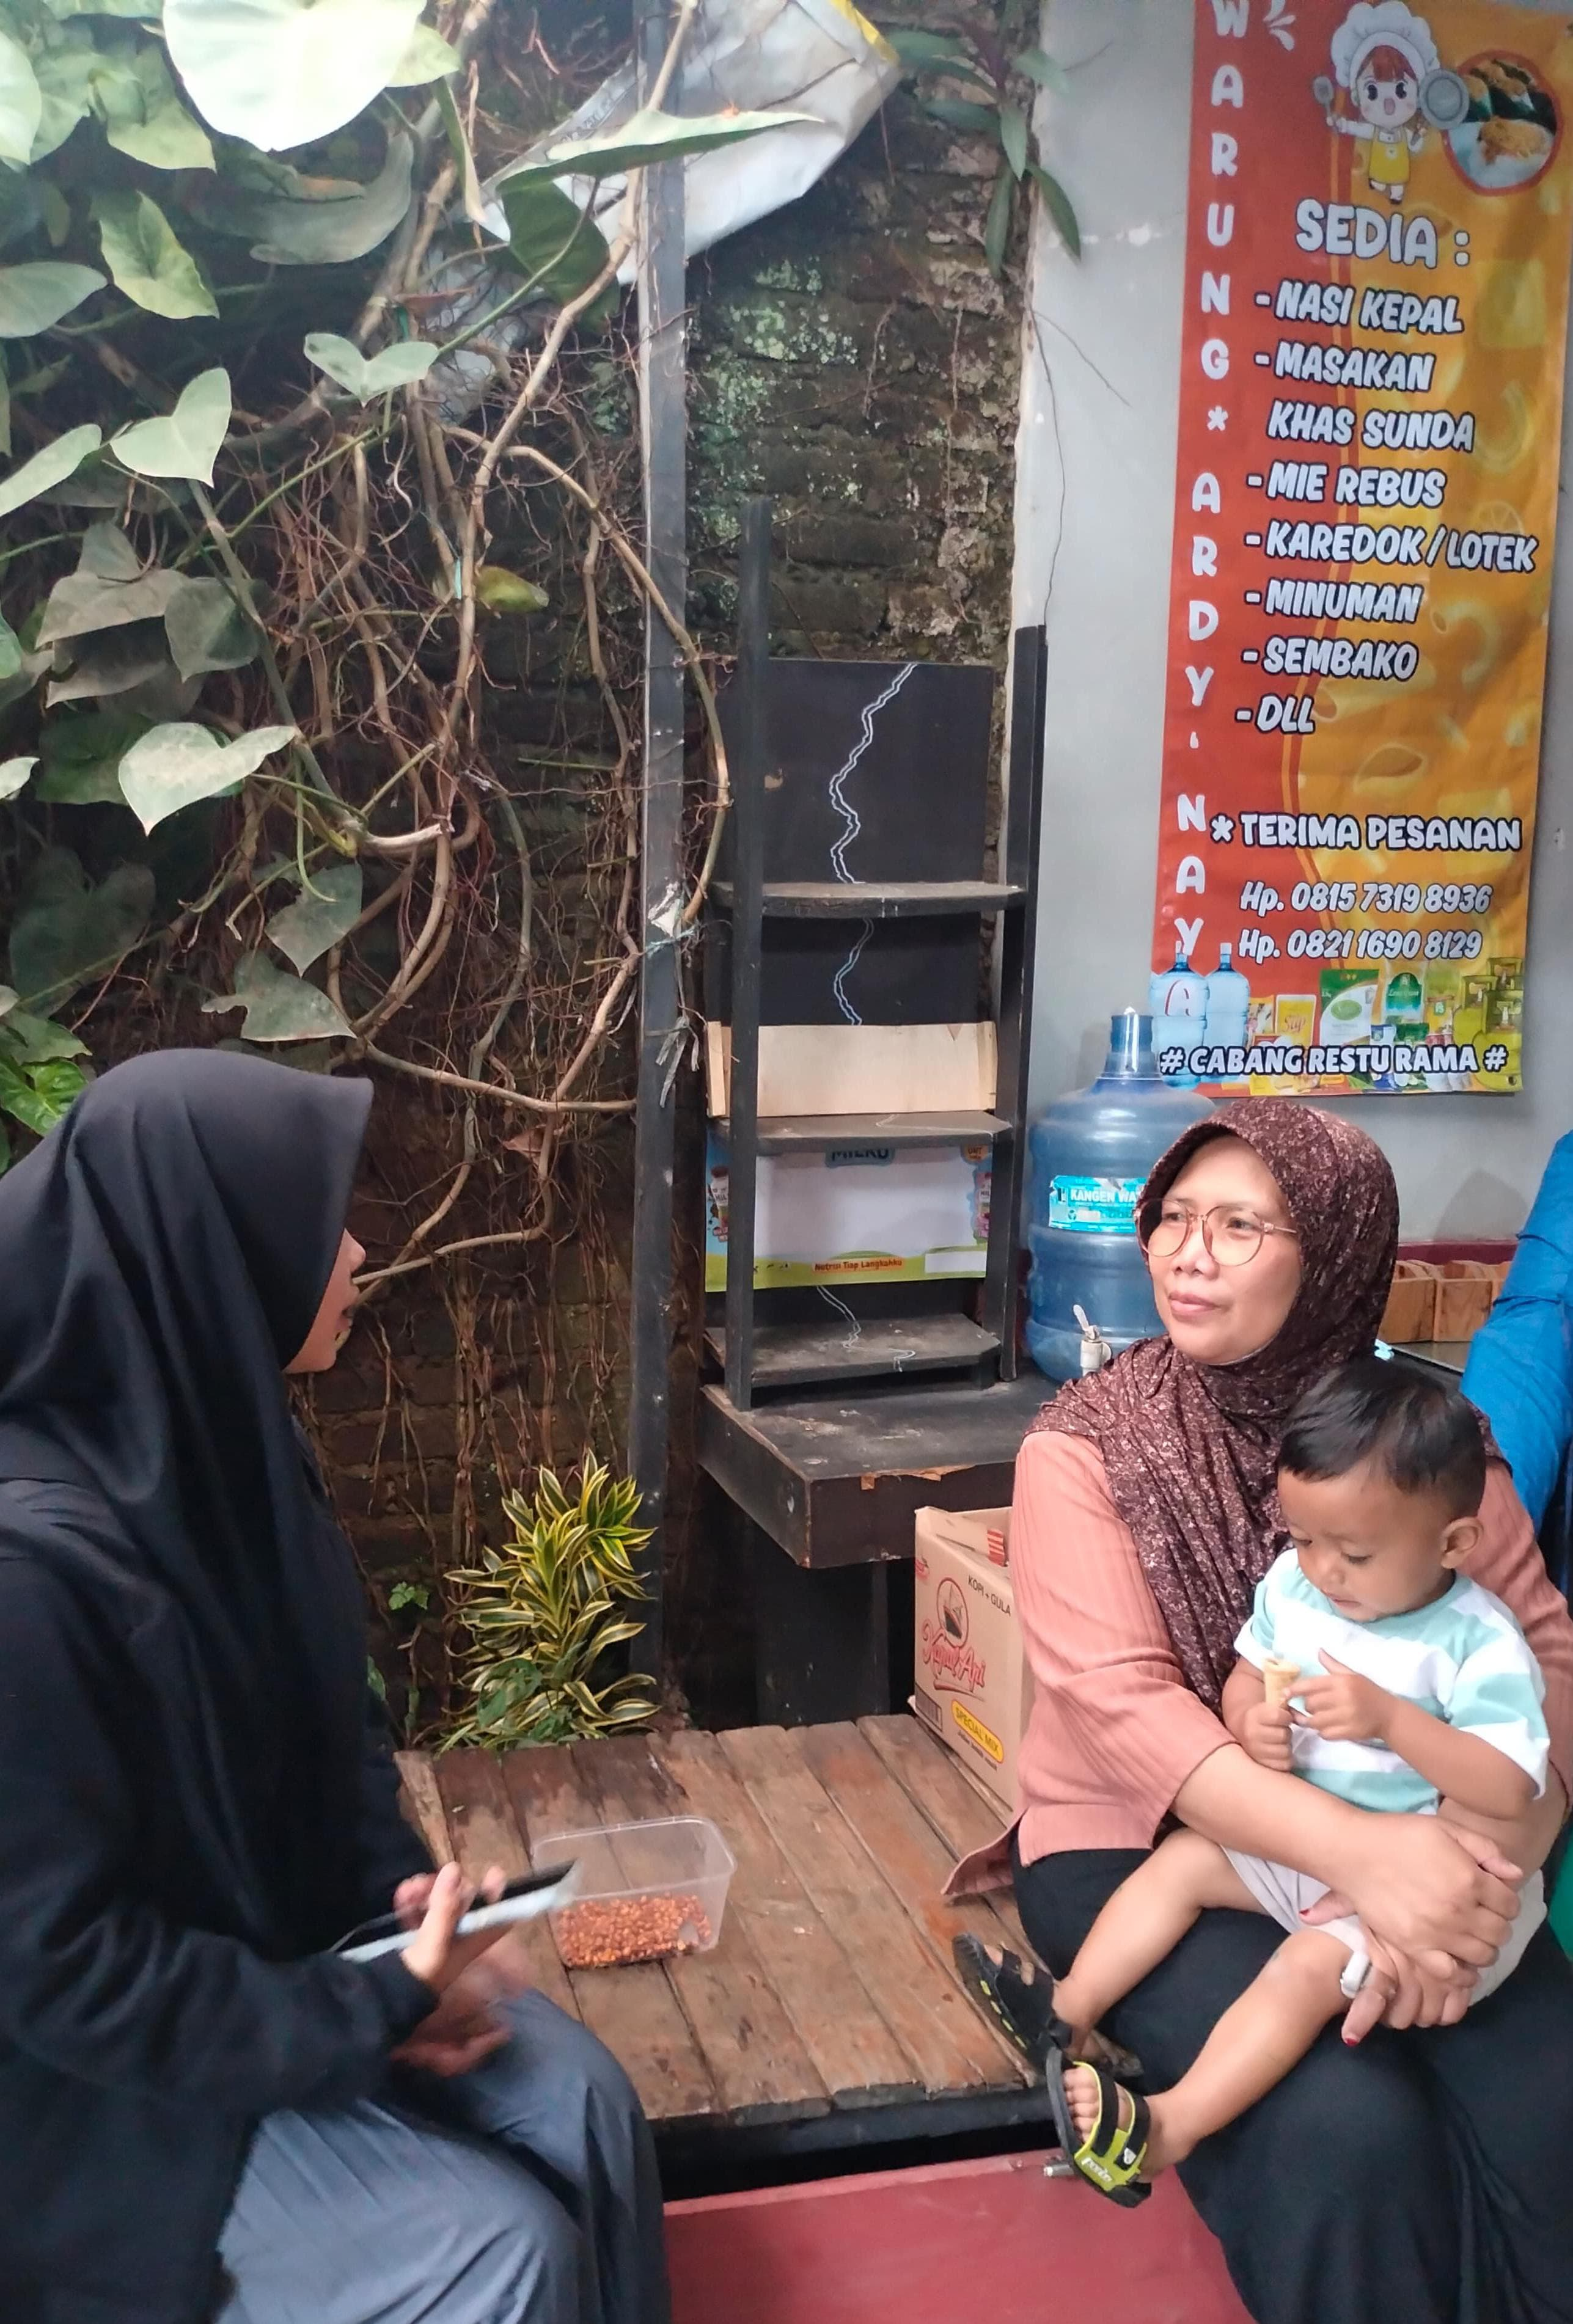
\includegraphics[width=0.4\textwidth]{images/gambar3.jpeg}
  \end{center}
\end{figure}
\begin{figure}[H]

  \begin{center}
    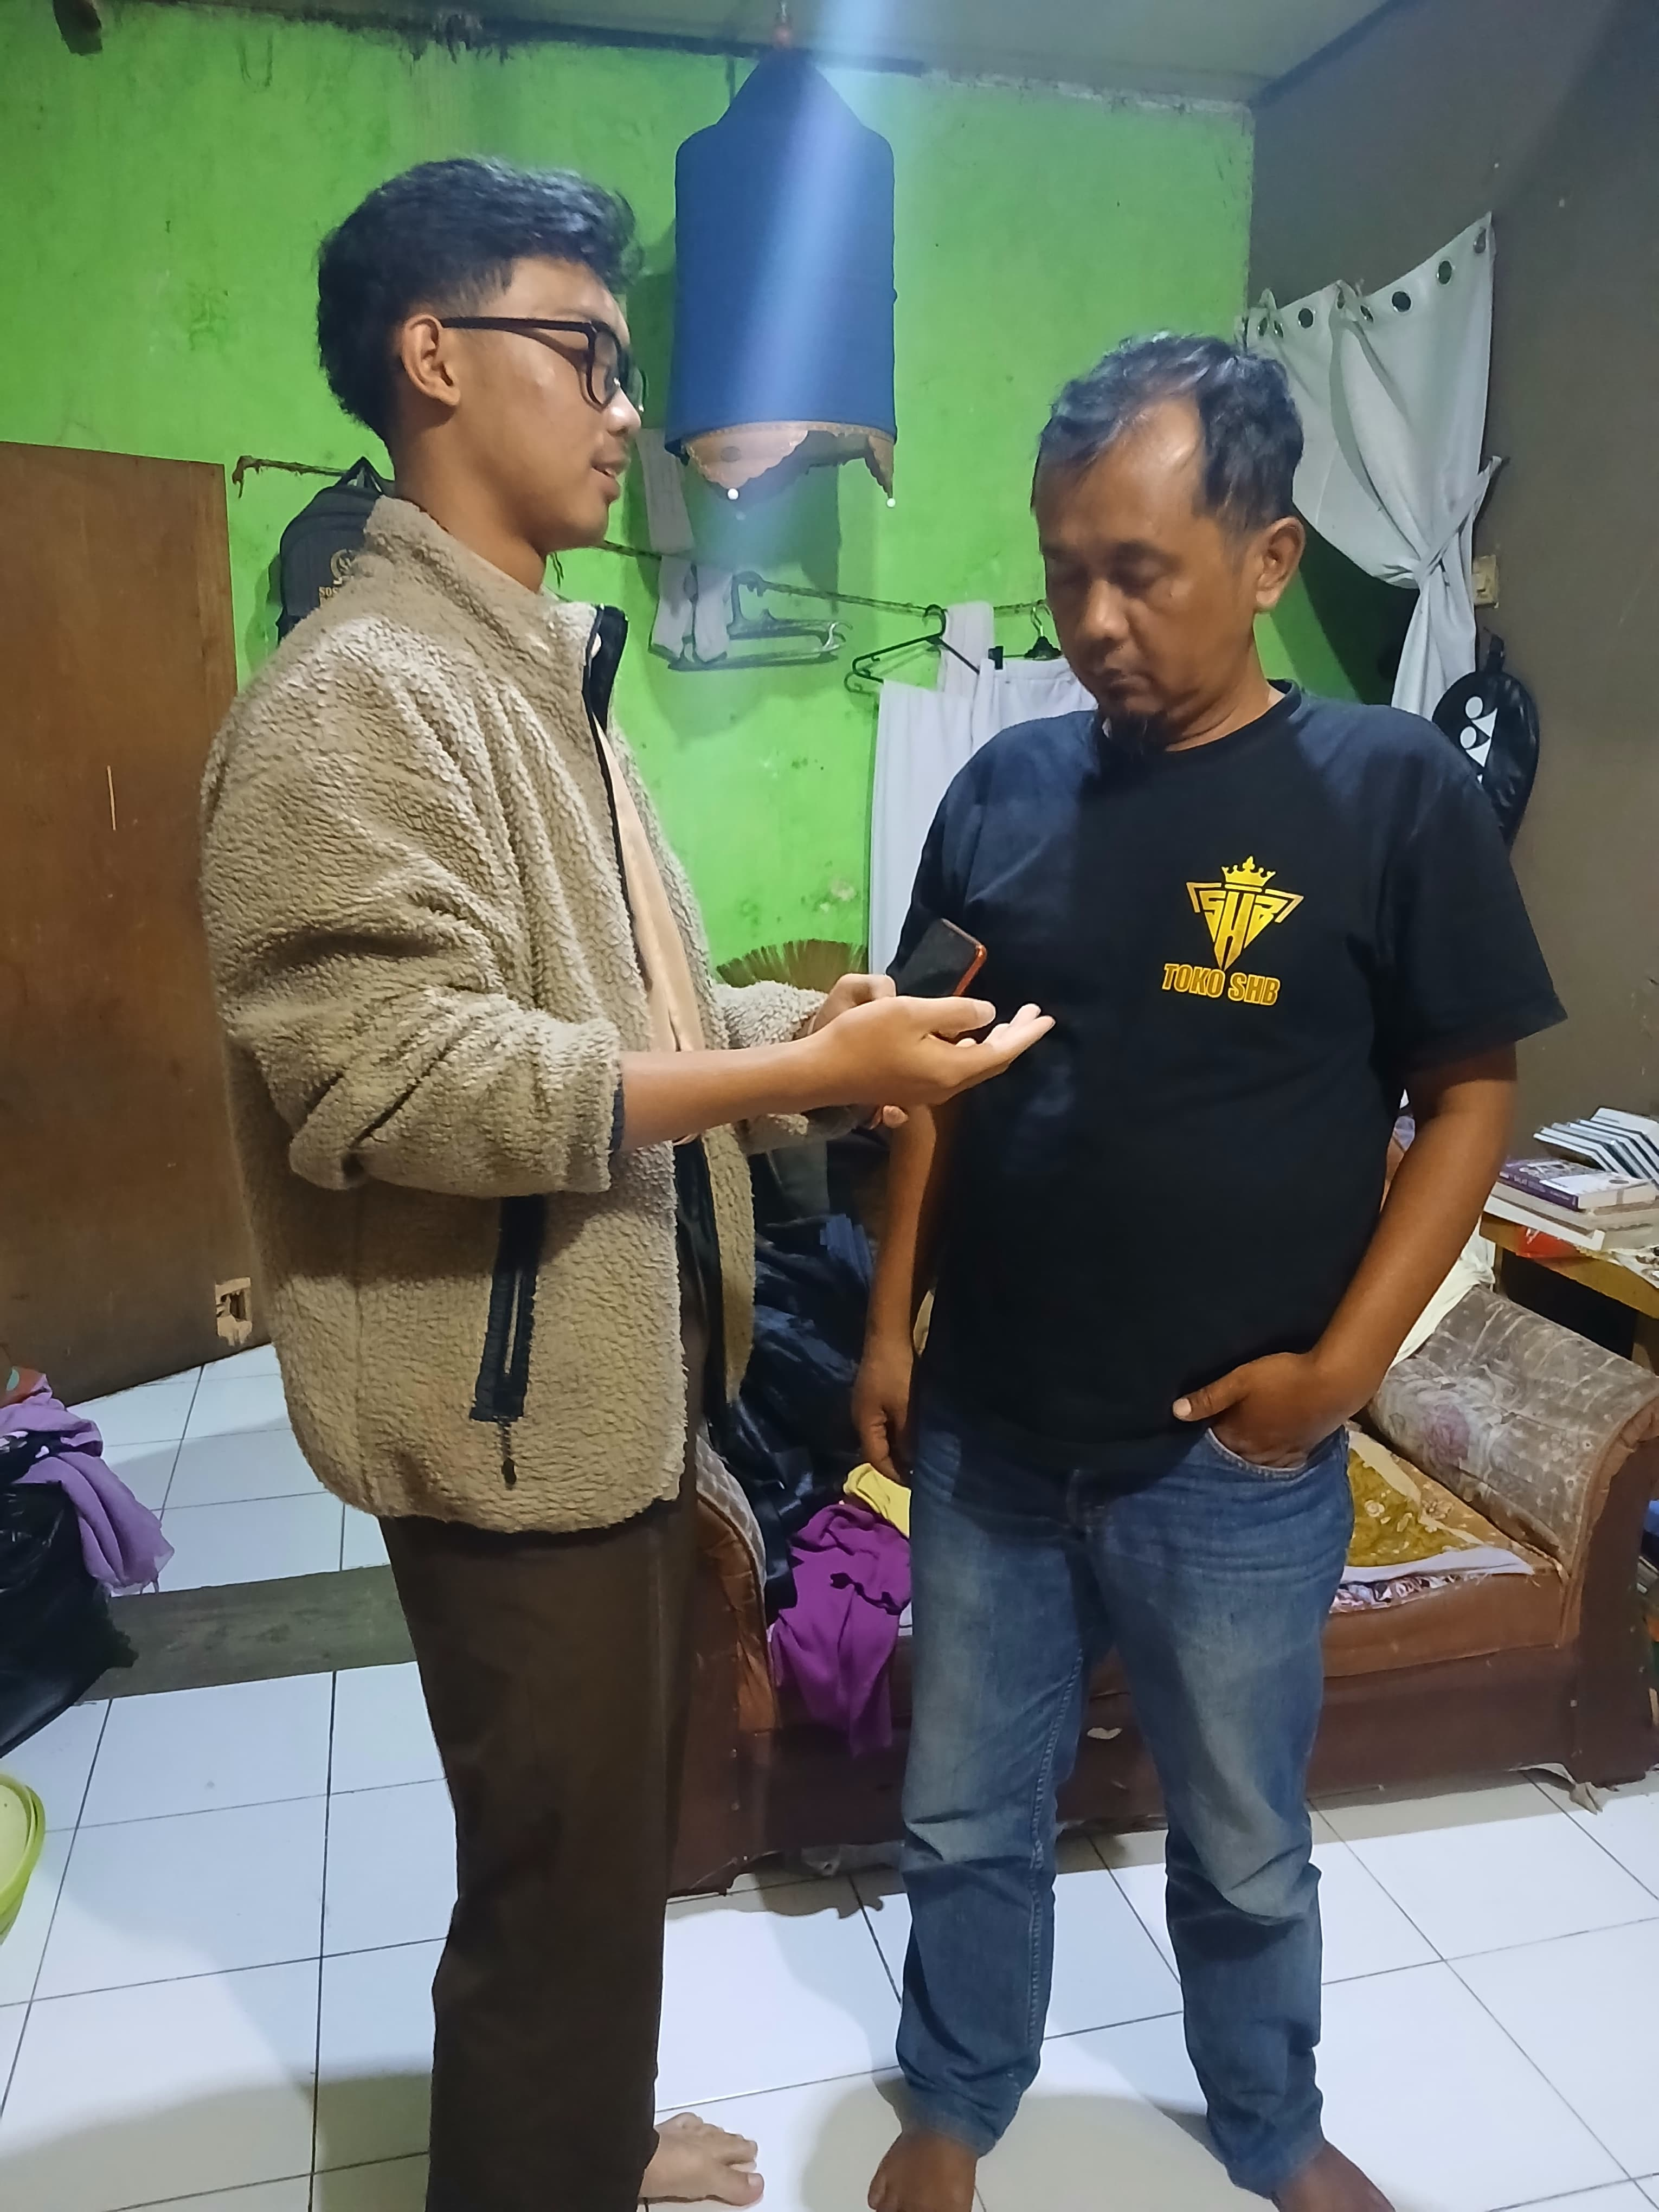
\includegraphics[width=0.4\textwidth]{images/gambar4.jpeg}
  \end{center}
\end{figure}
\begin{figure}[H]

  \begin{center}
    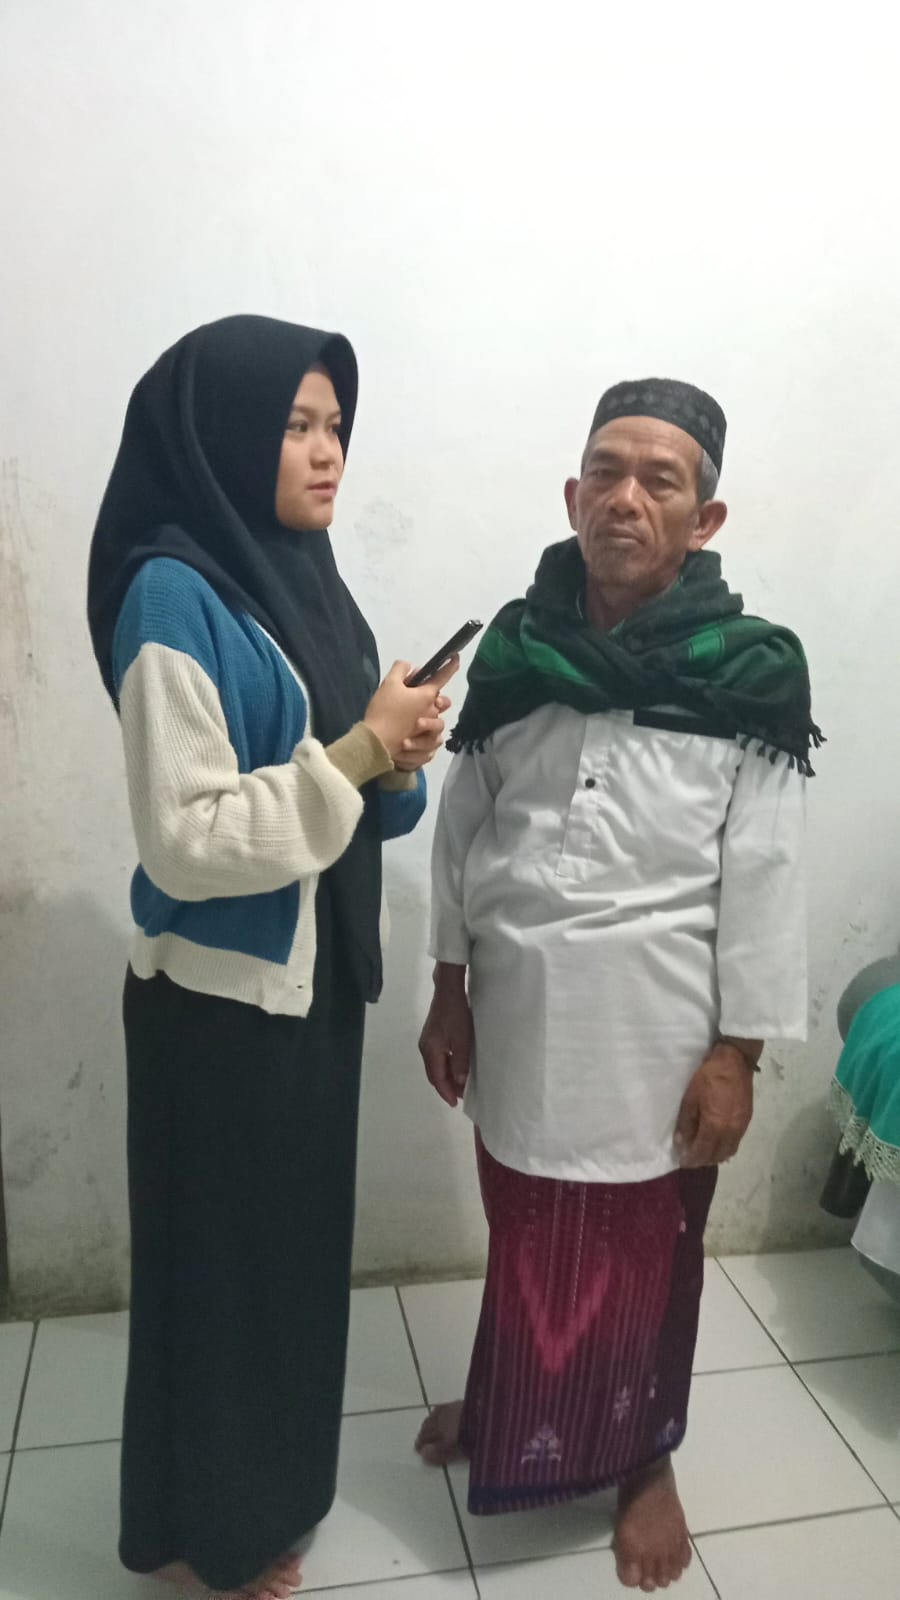
\includegraphics[width=0.4\textwidth]{images/gambar5.jpeg}
  \end{center}
\end{figure}
\begin{figure}[H]
  \begin{center}
    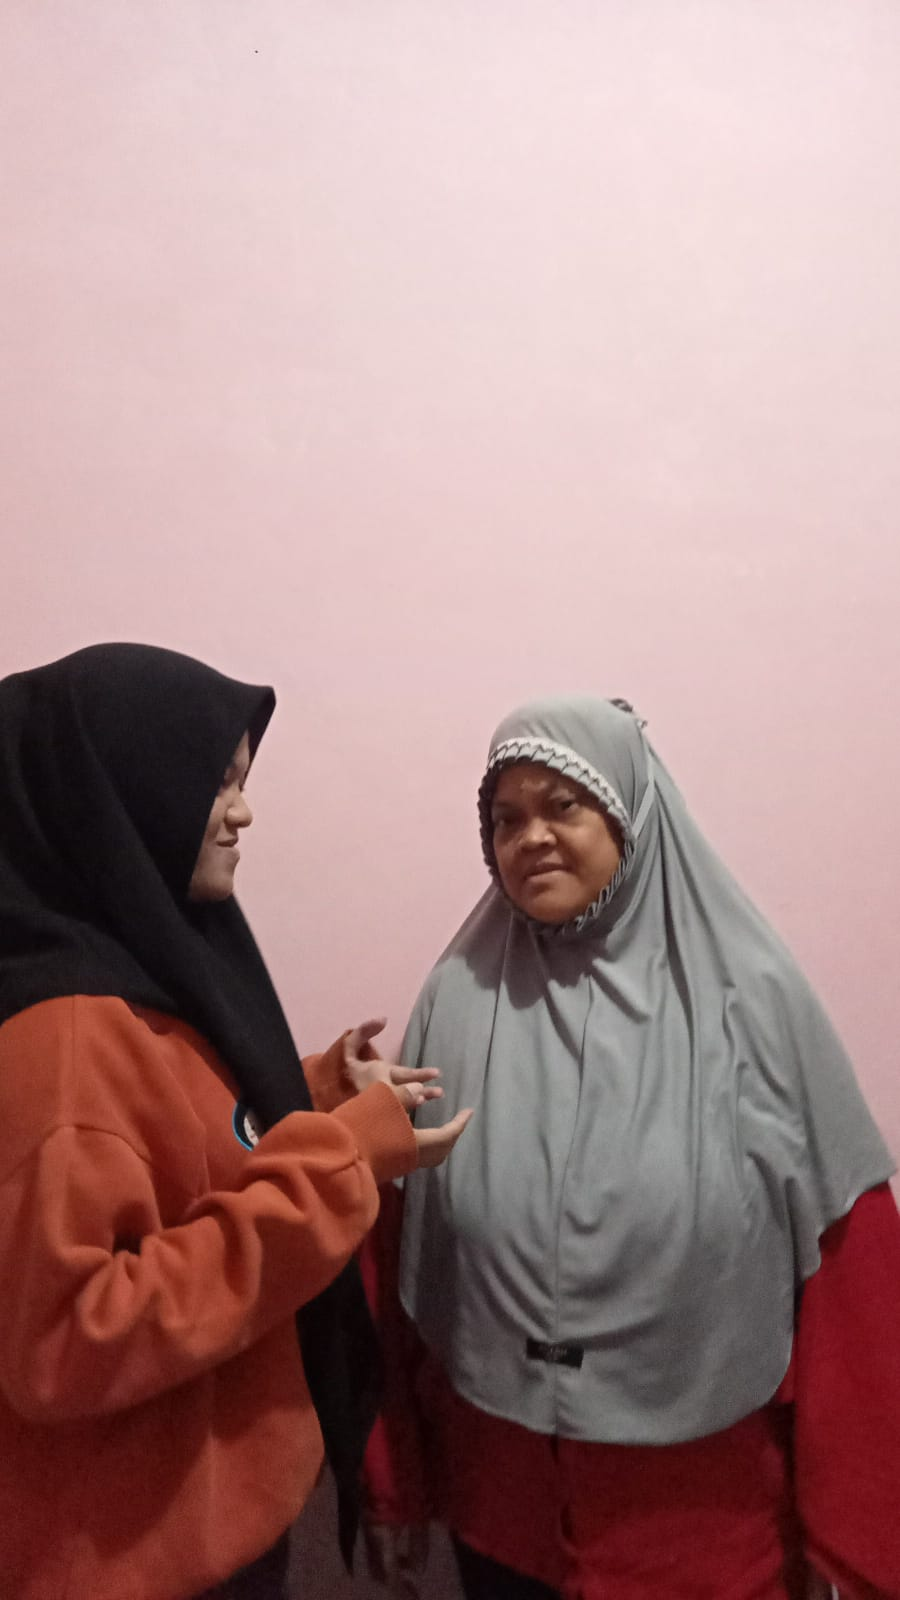
\includegraphics[width=0.4\textwidth]{images/gambar6.jpeg}
  \end{center}
\end{figure}


\setcounter{subsection}{0}
\setcounter{section}{5}
\section*{BAB IV \\ Kesimpulan dan Saran}
\addcontentsline{toc}{section}{\protect\numberline{}BAB IV Penutup}
\subsection{Kesimpulan}
ntegrasi kelompok minoritas di Ciwidey ditandai oleh pola koeksistensi tidak setara, di mana minoritas mampu bertahan secara kultural namun memiliki akses terbatas dalam pengambilan keputusan publik. Faktor ekonomi dan keberlanjutan lingkungan (khususnya pasca-bencana) menjadi determinan utama keberhasilan adaptasi, sebagaimana terlihat dalam studi hunian sementara pasca-bencana \cite{Priyo:2012}
% ciite this shit https://lib.ui.ac.id/file?file=digital%2Fold28%2F20305064-T30704+-+Hubungan+pola.pdf
\subsection{saran}
Berdasarkan dari Observasi kami, maka kami dapat memberikan beberapa saran yakni:
\begin{enumerate}
  \item Penguatan peran BUMDes dalam pemerataan kesempatan ekonomi antar kelompok
  \item Penyusunan protokol kesehatan hunian darurat yang mempertimbangkan aspek privasi dan budaya
  \item pembentukan sekolah lintas budaya untuk mempromosikan literasi multikultural sejak dini 
  \item optimalisasi forum dialog antar umat beragama yang ada di daerah sunda 
\end{enumerate}
Laporan ini menunjukkan bahwa harmonisasi sosial di Ciwidey bukanlah proses pasif, tetapi memerlukan intervensi kebijakan yang sensitif terhadap keragaman dimensi adaptasi kelompok minoritas
\addcontentsline{toc}{section}{\protect\numberline{}Daftar Pustaka}
\begin{thebibliography}{1}

\bibitem{Priyo:2012} 
Priyo. (2012). \textit{Hubungan Pola Adaptasi Akibat Bencana Terhadap Pemenuhan Kebutuhan Seksual pada Keluarga di Hunian Sementara Pasca Bencana Merapi Kabupaten Magelang} (Tesis, Universitas Indonesia).
\bibitem{Admin:2005}
Admin. (2005, November 21). Problem Mayoritas dan Minoritas dalam Interaksi Sosial. Diambil dari \url{https://balitbangdiklat.kemenag.go.id/berita/problem-mayoritas-dan-minoritas-dalam-interaksi-sosial}

\end{thebibliography}
\end{document}
